\documentclass{article}
\usepackage[utf8]{inputenc}
\usepackage{graphicx}
\graphicspath{{images/}{../images/}}
\usepackage{listings}

\title{Operating Systems Notes}
\author{Jacob Burley} %add your name here if you're a collaborator
\date{12 December 2017}

\begin{document}
\maketitle
\section{Introduction}
Operating System runs in kernel mode (supervisor mode), User programs run in User Mode
\\Instructions that control the machine or use I/O aren't available to User Mode (at least not directly)
\begin{center}
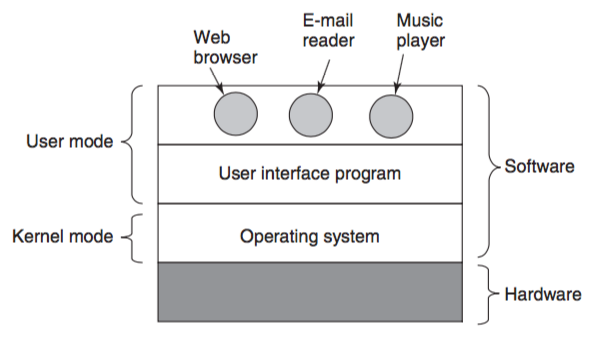
\includegraphics[width= 250pt]{tex/ch1/1-1.png}
\end{center}
\\Operating System runs on bare hardware
\\OS extends hardware of a computer, and makes it easier for programmers to develop applications without having to deal with things like SATA interfaces directly
\\OS also provides abstractions for devices, files etc.
\begin{center}
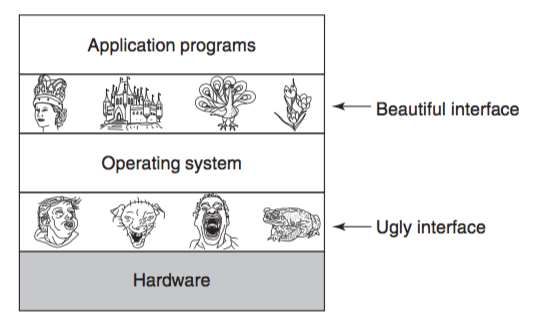
\includegraphics[width = 250pt]{tex/ch1/1-2.png}
\end{center}
\\OS also manages hardware resources like CPU and RAM, as well as I/O
\subsection*{First Generation Computers}
Earliest (first generation) computers didn't have an OS, were manually programmable using absolute machine language or physically rewiring plugboards to control basic functions of the machine
\subsection*{Second Generation Computers}
used transistors, became much more reliable
\\Batch systems involved collecting jobs on punchcards, reading them onto magnetic tape using a dedicated machine for this purpose, using this magnetic tape as input on the main computing machine, and then taking the output tape of that machine to another dedicated machine that printed the contents of the output tape
\\Structure of input job
\begin{itemize}
	\item \$JOB card, specifies maximum runtime in minutes, account number to be charged and programmer name
	\item \$FORTRAN card tells machine to load the FORTRAN compiler from the system tape, directly followed by program to be compiled
	\item \$LOAD card directed machine to load the object program that was just compiled
	\item \$RUN card, telling machine to run the program with the data that followed (like run-time arguments)
	\item \$END card marks the end of a job
\end{itemize}
used mostly for scientific and engineering calculations
\\They were largely programmed in FORTRAN and assembly
\\Typical OSes were the FORTRAN Monitor System, and IBM's IBSYS
\subsection*{Third Generation Computers}
Prior to 3rd gen, there were both large scale, word-oriented scientific computers but also character-oriented commercial computers
\section{Processes and Threads}

\section{Memory Management}

\section{File Systems}

\section{Input/Output}
OS controls a computers I/O
\\This involves issuing commands, catching interrupts and handling errors
\\OS should also provide a simple interface between devices and the rest of the system (to avoid horrible interfaces as in chapter 1)

\section{Deadlocks}
Systems have lots of resources that can only be used by one process at a time
\\We can't allow multiple processes to access a resource like a printer because it will lead to gibberish being printed
\\As a result, we allow a single process at a time to use resources like this
\\If process A requests a resource 1, and process B requests a resource 2, they are both granted these resources. If process A then requests resource 2 at the same time that process B requests resource 1, there will be a deadlock. Neither process will give up their currently held resource until they hold their newly requested resource, which means that neither process can advance.
\\
\\We have two types of resources: \textbf{preemptable}, and \textbf{Non-premptable}
\\\textbf{Preemptable} resources can be taken away from a process and given to another process without any ill effects. An example of this would be memory, as if a new process needs memory that an existing process occupies, then the memory that the existing process is using can simply be swapped out to disk, and the new process can take its place.
\\\textbf{Non-premptable} resources cannot be taken away from its current owner without potentially causing a failure. A device like a printer or a disk drive are examples of non-premptable resources
\\\textbf{non-premptable resources} are generally involved in deadlocks
\\deadlocks involving \textbf{preemptable resources} can usually be solved by reallocating resources
\\We assume that the sequence of events that all processes follow to use a resource is as follows
\begin{enumerate}
	\item Request the resource
	\item Use the resource
	\item Release the resource
\end{enumerate}
If a resource is not available on request, process may have to wait, may be blocked until it is available (depending on OS), or may receive an error code, in which case it can try again
\\Some kinds of resources (such as entries in a database) may be managed by the user processes themselves instead of the system, using semaphores or mutexes
\begin{lstlisting}[language=C]
/*
 * Using a semaphore to protect a single resource
 */
typedef int semaphore;
semaphore resource_1;

void process_A(void){
	down(&resource_1);
	use_resource_1();
	up(&resource_1);
}

/*
 * Using a semaphore to protect two resources
 */
typedef int semaphore;
semaphore resource_1;
semaphore resource_2;

void process_A(void){
	down(&resource_1);
	down(&resource_2);
	use_both_resources();
	up(&resource_2);
	up(&resource_1)
}
\end{lstlisting}
\textbf{Deadlock Definition:} \textit{A set of processes is deadlocked if each process in the set is waiting for an event that only another process in the set can cause.} 
\\4 conditions that must be present for resource deadlock to occur
\\each of these conditions represent a policy that may or may not be a characteristic of a given system
\\if one of the below is not present, no resource deadlock is possible
\begin{enumerate}
	\item Mutual exclusion condition: each resource is either currently assigned to exactly one process, or is available
	\item Hold-and-wait condition: processes currently holding resources that were granted earlier can request new resources
	\item No-preemption condition: Resources previously granted cannot be forcibly taken away from a process. They must be explicitly released by the process holding them
	\item Circular wait condition: There must be a circular list of two or more processes, each of which is waiting for a resource held by the next member of the chain
\end{enumerate}
We can model resources (and thus deadlocks) as shown in the diagram below
\begin{center}
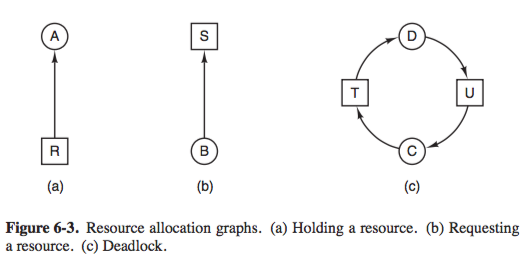
\includegraphics[width= 250pt]{tex/ch6/6-3.png}
\end{center}
Cycles like in c) mean that there is a deadlock, as the processes cannot break out of that loop.
There are four strategies for dealing with deadlocks:
\begin{enumerate}
	\item Just ignore the problem (Ostrich Algorithm)
	\item Detection and Recovery: Wait until they occur, then detect them and take action
	\item Dynamic avoidance by careful resource allocation
	\item Prevention, by structurally negating one of the four conditions mentioned above
\end{enumerate}
\subsection*{Ostrich Algorithm}
\\acceptable as a solution if deadlocks are rare
\subsection*{Detection and recovery}
\\implemented differently for different scenarios. With unique resources of each type, we can create a resource graph and look for cycles. If there are cycles, the system is deadlocked, otherwise it is not. There is also an algorithm for detecting cycles in a resource graph (useful, as an OS doesn't have eyes)
\begin{enumerate}
	\item For each node $N$ in the graph, perform the following five steps with $N$ as the starting node
	\item Initialize $L$ as an empty list, and designate all the arcs as unmarked
	\item Add the current node to the end of $L$ and check to see if the node now appears in $L$ two times. If it does, the graph contains a cycle (listed in $L$) and the algorithm terminates
	\item From the given node, see if there are any unmarked outgoing arcs. If so, go to step 5; if not, go to step 6
	\item Pick an unmarked outgoing arc at random and mark it. Then, follow it to the new current node and go back to step 3
	\item If this node is the initial node, the graph does not contain any cycles and the algorithm terminates. Otherwise, we have reached a dead end. Remove it, and go back to the previous node (the one that was the current node \textbf{before} this one), make that the current node, and go to step 3.
\end{enumerate}
This algorithm takes each node in turn, as the root of what it hopes will be a tree, and does a depth-first search on it. If it ever comes back to a node that is already in $L$, that means there is a cycle. When it exhausts all the arcs for a given node, it backtracks to the previous node. If it backtracks to the root of the tree (and thus cannot go further), the subgraph reachable from the current node does not contain any cycles. If this property holds for all nodes, the entire graph is cycle free and the system is \textbf{not deadlocked}.
\\There are 3 ways of recovering from a deadlock after detecting it
\begin{enumerate}
	\item Preemption: It may be possible to temporarily take a resource away from its current owner, and give it to another process. In many cases, manual intervention may be required (especially batch-processing OSes on mainframes). The ability to do this is dependent on the nature of the resource in question, and is frequently difficult or impossible. Choosing the process to suspend is mostly dependent on which ones have resources that can easily be taken away
	\item Rollback: if the system designers know that deadlocks are likely, they could arrange to checkpoint processes periodically. Checkpointing involves writing the process state to a file periodically. Checkpoint contains memory image and resource state (which resources are currently assigned to which processes). For maximum effectivity, we don't overwrite old checkpoints when we create new ones. 
	\\When a deadlock is detected, we can see which resources are needed easily. To recover from the deadlock, we can roll back a process that owns a needed resource to a point in time when it didn't own that resource. All the work done by this process since that checkpoint is lost, but the deadlocked process can continue. If the process that was rewound tries to acquire that resource again, it will have to wait until it becomes available.
	\item Killing processes: A crude but simple recovery method. You could start by killing processes in a cycle until the cycle is broken. Alternatively, a process \textbf{not} in the cycle could be chosen, if it holds resources that a process in the cycle might need to continue. 
	\\Ideally, we kill processes that can be run again from the beginning with no negative effects. Compiling is a good example, as killing a compile process midway has no influence on the source file it compiled from, thus has no influence on the results of running it a second time. \textbf{Killing processes that aren't idempotent is not a good idea.} You do not want to add duplicate results to a database by killing the program writing to the database halfway through its first operation.
\end{enumerate}
\subsection*{Deadlock Avoidance}
\\processes usually ask for their desired resources one at a time. The OS must determine whether granting that resource is safe or not, and do so only if the grant is safe. It is thus possible to make an algorithm that avoids deadlocks by always allocating in a safe way.
\\\textbf{Safe state:} There is some scheduling order in which every process is \textit{guaranteed} to run to completion even if all of them suddenly request their maximum number of resources immediately.
\begin{center}
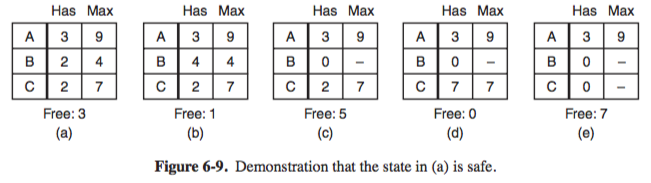
\includegraphics[width= 250pt]{tex/ch6/6-9.png}
\end{center}
\\An \textbf{unsafe state} is not a deadlocked state. Entering into an unsafe state may not lead to a deadlock for a little while, but not all of the processes will be able to complete as they will enter a deadlocked state at some point.
\\Luckily, Dijkstra (of algorithm fame) created a scheduling algorithm to avoid deadlocks, the \textbf{Banker's Algorithm}.
\subsubsection*{The Banker's Algorithm}
\begin{center}
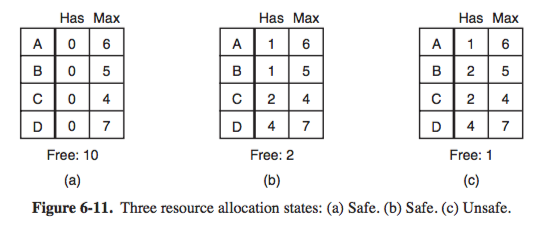
\includegraphics[width= 250pt]{tex/ch6/6-11.png}
\end{center}
The bankers Algorithm needs to know three things to work
\begin{enumerate}
	\item How much of each resource each process could possibly request (its MAX)
	\item How much of each resource each process is currently holding (ALLOCATED)
	\item How much of each resource the system currently has available (AVAILABLE)
\end{enumerate}
We can also assume a NEED value which is equal to $MAX - ALLOCATED$
\\Resources are only allocated if 
$$p_{MAX} \leq AVAILABLE$$
otherwise, the process waits until resources are available. The bank (the system) never allocates its resources (AVAILABLE) in such a way that AVAILABLE would be less than any of its customers MAX - ALLOCATED. This works because if the system needs a resource, it will satisfy the request that keeps the system in a safe state but also allows a process to complete. Upon completing, the process then yields its resources back to the system, so its AVAILABLE can grow.
\\We can also use the Banker's Algorithm for multiple resources.
\begin{center}
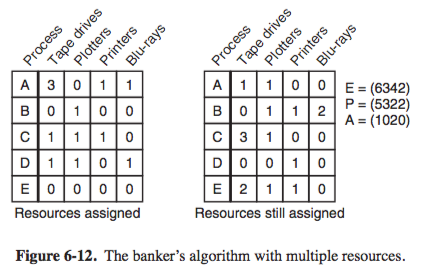
\includegraphics[width= 250pt]{tex/ch6/6-12.png}
\end{center}
In the above diagram, we can see a matrix on the left showing which resources are already allocated to a set of processes, and a matrix on the right showing what resources those processes still need in order to complete. Processes state their total resource needs before executing, so the system can compute the right hand matrix constantly.
\\On the right, there are 3 vectors: $E$ (existing resources), $P$ (possessed resources) and $A$ (available resources).
\\Knowing these vectors and what they mean, we can now understand the algorithm.
\begin{enumerate}
	\item Look for a row, $R$, whose unmet resource needs are all less than or equal to $A$. If a row that meets these conditions doesn't exist, the system will eventually deadlock since no process can complete (assuming processes keep all resources until they exit)
	\item Assume the process of the chosen row requests all the resources it needs (which is guaranteed to be possible) and finishes. Mark that process as terminated, and add all of its resources to the $A$ vector
	\item Repeat steps 1 and 2 until either all processes are marked as terminated (the initial state was safe) or no process is left whose resources needs can be met (in which case the system was not safe)
\end{enumerate}
If several processes are eligible to be chosen in step 1, we can choose at random. $A$ either gets larger, or in the worst case, it stays the same.
\\In practice, very few systems use the Banker's Algorithm to avoid deadlocks. Processes in most systems do not know the type or amount of resources that they will need in advance. Resources can also suddenly vanish (if a drive breaks, for example)
\subsection*{Deadlock Prevention} 
we can try and stop one of the four conditions for deadlocks from happening
\subsubsection*{Attacking the mutex condition}
if no resource were ever assigned to just a single process, we would never have deadlocks
\\For data, we can make it all read only, so all processes can use it at the same time
\\we can spool output for devices like printers so that multiple processes can generate output at the same time without interfering with eachother
\\we use a printer daemon to actually request printer access, which it usually does after the complete output file from a process is spooled
\\We \textbf{could} get a deadlock if two processes had filled the spool but weren't finished with their output, at which point neither process can continue printing to the spool and the daemon cant send a job to the printer.
\\However, the basic concept of this technique is still usable: avoid assigning resources unless absolutely necessary, and try to make sure that as few processes as possible may actually claim the resource
\subsubsection*{Attacking Hold-and-wait}
Seems like the obvious answer, because if we can prevent processes from holding resources while they request resources, deadlocks would be gone.
\\One way to achieve this could be asking all processes to declare all the resources they need before executing. If everything is available at that time, it can execute. Otherwise, it waits
\\This doesn't work because processes frequently have no idea what they will need before they need it. If they knew, we could actually use the banker's algorithm!
\\Some mainframe batch systems do actually require processes to do this, which is inefficient, but does prevent deadlocks
\\We can also break the hold-and-wait condition by requiring processes requesting a resource to first temporarily release all the resources it currently holds. It then tries to get everything it needs all at once
\subsubsection*{Attacking No-Preemption}
We would struggle to take the printer away from a process suddenly, but we could virtualize resources so we don't have to.
\\We could spool printer output to disk, and only allow the printer daemon access to the printer eliminates printer deadlocks, but could introduce potential hard disk deadlocks
\\We can't virtualize all resources like this though
\\Records in a DB or tables in an OS must be locked to be used, which can lead to deadlocks.
\subsubsection*{Attacking Circular Wait}
Could have a rule preventing a process from having more than 1 process at any moment. This would inhibit a process copying data between two devices (from a tape to a printer, for example)
\\We could also provide \textbf{global numbering} of all resources. Now, the rule should force processes to make all of their resource requests in numerical order
\\With this rule, a resource allocation graph will never have cycles, as processes cannot request resources that other processes have requested
\\At each instant, one of the assigned resources will have the highest number. The holding process can't ask for a number lower than the one it has (they are potentially already assigned anyways), and they can ask for any higher number because all of those would be unassigned. Alternatively, the process could finish. Another process then holds the highest assigned number, and then this process will finish etc. No deadlocks, and every process can finish
\\A variation of this algorithm drops the requirement that processes request a resource with a \textbf{higher number}, instead mandating that they cannot request a resource lower than it is already holding. If the process drops their held resource, they can request any resource they want.
\\This numerical ordering eliminates deadlocks, but it may be impossible to find an ordering to satisfy everyone. The number of potential resources and uses for these resources means that there isn't an ordering that works, so this method is also not used.
\subsection*{Livelock}
Processes can be polite by giving up locks it already has if it notices it cannot obtain its next lock. Then, it waits a millisecond and tries again. This seems like it could help resolve deadlocks, but actually it can cause the opposite. If another process does the same thing at the same time, this creates a situation where both processes yield to eachother, and no progress is made because neither of them end up with the extra resource they needed
\subsection*{Starvation}
\textbf{Process starvation} is closely related to dead/livelocks
\\How do we allocate a high-demand resource so that processes don't starve?
\\We could give it to the program with the smallest task (i.e. smallest file to print), but this would starve processes with large tasks, as they will not be prioritised
\\So we use a first come, first serve allocation policy, because all processes will eventually become the oldest and get the resource.
\end{document}